\documentclass[11pt]{article}

\usepackage[margin=1in]{geometry}
\usepackage{graphicx}
\usepackage{booktabs}
\usepackage{float}
\usepackage{hyperref}
\usepackage{listings}
\usepackage{xcolor}
\usepackage{titling}
\usepackage{fancyhdr}
\usepackage{amsmath}

\hypersetup{colorlinks=true, linkcolor=blue, citecolor=blue, urlcolor=blue}

\lstset{
  basicstyle=\ttfamily\small,
  breaklines=true,
  frame=single,
  backgroundcolor=\color{gray!10},
  keywordstyle=\color{blue},
  commentstyle=\color{gray},
  showstringspaces=false,
  language=Python
}

\pagestyle{fancy}
\fancyhf{}
\rhead{CS 3502 -- Project 2}
\lhead{CPU Scheduling Simulator}
\rfoot{\thepage}

\title{\vspace{-1.5cm}\textbf{CPU Scheduling Simulator} \\ \large Performance Analysis and Algorithm Comparison \\ \normalsize OwlTech Industries -- Performance Optimization Division}
\author{Bryce Wendell Jones \\ CS 3502: Operating Systems \\ Department of Computer Science \\ Kennesaw State University}
\date{\today}

\begin{document}

\maketitle
\thispagestyle{empty}
\newpage

\tableofcontents
\newpage

% =========================================================================
\section{Introduction}
% =========================================================================

This report documents the design, implementation, and empirical evaluation
of a CPU scheduling simulator built for CS 3502 Project 2. Following the
``Hybrid'' option described in the assignment, the algorithm logic was
implemented from scratch in Python and paired with a Streamlit-based web
interface rather than extending the provided C\# starter project.

The simulator implements six scheduling algorithms: the four required by
the starter specification --- First-Come First-Served (FCFS), Shortest Job
First (SJF), Round Robin (RR), and Priority scheduling --- plus two
additional algorithms selected from the assignment's approved list:
Shortest Remaining Time First (SRTF) and Multi-Level Feedback Queue (MLFQ).

The goal, framed by the assignment's narrative, is to give OwlTech
Industries' Performance Optimization Division a data-driven recommendation
for which scheduling approach best serves its production workloads, which
mix CPU-bound, I/O-bound, and mixed process types at small, medium, and
large scale.

% =========================================================================
\section{Software Architecture}
% =========================================================================

\subsection{Design Philosophy}

The codebase separates three concerns that are easy to tangle together in a
scheduling simulator: (1) the data model for a process/PCB, (2) the
scheduling algorithms themselves, and (3) the presentation layer (web UI,
charts, CSV export). Each algorithm is a pure function of the form
\texttt{run(processes) -> SchedulingResult}, which makes every algorithm
independently testable and prevents one algorithm's state from leaking into
another's.

\subsection{Directory Structure}

\begin{lstlisting}[language=]
assignment4/
|-- app.py                     Streamlit web interface
|-- requirements.txt
|-- README.md
|-- generate_report_figures.py Regenerates report figures from live code
|-- report/
|   |-- report.tex             This document
|   |-- references.bib
|   |-- results_tables.tex     Auto-generated result tables (real data)
|   `-- figures/               Gantt charts, comparison charts, screenshots
|-- src/
|   |-- process.py             Process / PCB data structure
|   |-- scheduler.py           Algorithm dispatcher
|   |-- metrics.py             AWT, ATT, CPU util., throughput, response time
|   |-- workload_generator.py  Reproducible small/medium/large workloads
|   |-- visualization.py       Plotly Gantt & comparison charts
|   |-- utils.py               Validation, CSV export
|   `-- algorithms/
|       |-- fcfs.py
|       |-- sjf.py
|       |-- round_robin.py
|       |-- priority.py
|       |-- srtf.py            (new algorithm)
|       `-- mlfq.py            (new algorithm)
|-- data/                      Generated sample workloads (CSV)
|-- results/                   Generated per-run results and comparisons
`-- tests/
    `-- test_algorithms.py     36 unit tests
\end{lstlisting}

\subsection{Process (PCB) Data Structure}

Every process is represented by the \texttt{Process} dataclass in
\texttt{src/process.py}. It separates \emph{static} attributes set at
creation (pid, arrival time, burst time, priority, process type) from
\emph{dynamic} attributes a scheduler fills in during simulation
(remaining time, start time, completion time, waiting time, turnaround
time, response time, execution history). A \texttt{clone()} method
produces an independent copy of a workload so that running six algorithms
against the same process table never lets one algorithm's mutations affect
another's results.

\subsection{Scheduler Dispatch}

\texttt{src/scheduler.py} defines \texttt{Scheduler}, a thin registry that
maps an algorithm name (e.g. \texttt{"SRTF"}) to its implementation
function and clones the workload before each run. This keeps \texttt{app.py}
and the test suite decoupled from the individual algorithm modules.

% =========================================================================
\section{Algorithm Implementations}
% =========================================================================

All six algorithms use \texttt{arrival\_time} and \texttt{burst\_time} to
determine execution order; behavior differs in whether they are
non-preemptive or preemptive, and what value they use to choose the next
process to run.

\subsection{First-Come, First-Served (FCFS)}
Non-preemptive. Processes run strictly in order of arrival time, ties
broken by process ID. It is the simplest possible policy and the baseline
every other algorithm is measured against. FCFS has no starvation risk but
suffers from the ``convoy effect'': a single long process can force many
short processes to wait, inflating average waiting time.

\subsection{Shortest Job First (SJF)}
Non-preemptive. When the CPU becomes free, the ready process with the
smallest \emph{total} burst time is selected next. SJF is provably optimal
for minimizing average waiting time among non-preemptive algorithms, but
requires knowing burst times in advance and can starve long processes
under continuous arrivals of short jobs.

\subsection{Round Robin (RR)}
Preemptive. Each process receives at most one time quantum (default 4
time units in this simulator) before being preempted and sent to the back
of the ready queue. RR guarantees fairness and low response time
regardless of burst length, at the cost of higher average waiting/
turnaround time versus SJF/SRTF, plus context-switch overhead that grows
as the quantum shrinks.

\subsection{Priority Scheduling}
Non-preemptive. The ready process with the numerically smallest priority
value (1 = highest priority) runs next, ties broken by arrival time then
process ID. This implementation does not use aging, so low-priority
processes can in principle starve under continuous high-priority arrivals;
this trade-off is discussed further in Section~\ref{sec:tradeoffs}.

\subsection{Shortest Remaining Time First (SRTF) --- New Algorithm}
Preemptive variant of SJF. At every time step, the ready process with the
smallest \emph{remaining} time runs; a newly arrived process preempts the
running process immediately if its burst is shorter than the running
process's remaining time. SRTF is the preemptive analogue of SJF and is
optimal for minimizing average waiting time among \emph{all} scheduling
policies (preemptive or not), at the cost of more context switches and,
like SJF, the theoretical possibility of starving long processes.

Implementation note: the simulator advances in unit time steps and
re-evaluates a min-heap of ready processes keyed on remaining time after
every unit, which keeps the preemption logic simple to verify by hand
while still handling 100+ process workloads in well under a second (see
Section~\ref{sec:testing}).

\subsection{Multi-Level Feedback Queue (MLFQ) --- New Algorithm}
Preemptive and adaptive. MLFQ uses three queues (default quanta 4, 8, 16
time units) with strict priority between levels and round robin within a
level. New processes enter at the highest-priority queue (level 0). A
process that consumes its entire quantum without finishing is demoted one
level (the scheduler infers it is more CPU-bound); a process that finishes
within its quantum completes without demotion. This lets MLFQ approximate
SJF-like behavior --- favoring short/interactive jobs --- without requiring
advance knowledge of burst times, which is the central practical advantage
MLFQ has over SJF/SRTF in a real operating system.

% =========================================================================
\section{Performance Metrics}
% =========================================================================

For every algorithm and workload, the simulator computes:

\begin{itemize}
  \item \textbf{Average Waiting Time (AWT):} mean time each process spends
    ready but not running.
  \item \textbf{Average Turnaround Time (ATT):} mean of
    (completion\_time $-$ arrival\_time) across all processes.
  \item \textbf{Average Response Time (ART):} mean of
    (first\_start\_time $-$ arrival\_time), i.e. how long a process waits
    before its \emph{first} CPU burst.
  \item \textbf{CPU Utilization:} percentage of the schedule's total
    makespan during which the CPU was not idle.
  \item \textbf{Throughput:} completed processes per unit simulated time.
\end{itemize}

All four metric formulas (AWT, ATT, CPU utilization, throughput) are
implemented in \texttt{src/metrics.py} and applied identically regardless
of which algorithm produced the schedule, so comparisons across algorithms
are apples-to-apples.

% =========================================================================
\section{Workload Design}
\label{sec:workloads}
% =========================================================================

Three size classes were generated, matching the assignment's testing
requirements:

\begin{itemize}
  \item \textbf{Small} (n=8): hand-verifiable; used for the FCFS/SJF/RR/
    Priority unit tests derived directly from the process table in the
    assignment PDF (Section 4.1).
  \item \textbf{Medium} (n=30): large enough for stable performance trends
    to emerge.
  \item \textbf{Large} (n=120): stress test for scalability.
\end{itemize}

Each size was generated in three workload-type variants:

\begin{itemize}
  \item \textbf{CPU-bound:} long bursts (10--30 time units), simulating
    compute-heavy processes.
  \item \textbf{I/O-bound:} short bursts (1--6 time units), simulating
    processes that spend most of their time blocked on I/O in a real
    system.
  \item \textbf{Mixed:} a roughly even mixture of CPU-bound, I/O-bound, and
    intermediate processes.
\end{itemize}

All workloads are generated by \texttt{src/workload\_generator.py} using
Python's \texttt{random.Random(seed)}, so any workload is exactly
reproducible given its (size, type, seed) triple --- every result in this
report used \texttt{seed=42}.

% =========================================================================
\section{Performance Evaluation}
\label{sec:evaluation}
% =========================================================================

\subsection{Comparison Tables}

Tables~\ref{tab:small_cpu_bound}--\ref{tab:large_mixed} report every metric
for all six algorithms across all nine (size $\times$ type) workload
combinations, generated directly from live simulation runs (not hand
estimates). AWT/ATT/ART are in simulated time units; throughput is in
processes per unit time.

\begin{table}[H]
\centering
\small
\begin{tabular}{lrrrrr}
\toprule
Algorithm & AWT & ATT & ART & CPU Util. (\%) & Throughput \\
\midrule
FCFS & 64.50 & 85.12 & 64.50 & 100.00 & 0.0485 \\
SJF & 57.12 & 77.75 & 57.12 & 100.00 & 0.0485 \\
Round Robin & 111.38 & 132.00 & 12.75 & 100.00 & 0.0485 \\
Priority & 74.00 & 94.62 & 74.00 & 100.00 & 0.0485 \\
SRTF & 57.12 & 77.75 & 57.12 & 100.00 & 0.0485 \\
MLFQ & 92.62 & 113.25 & 12.75 & 100.00 & 0.0485 \\
\bottomrule
\end{tabular}
\caption{Small Workload (CPU-bound, n=8) -- Algorithm Comparison}
\label{tab:small_cpu_bound}
\end{table}

\begin{table}[H]
\centering
\small
\begin{tabular}{lrrrrr}
\toprule
Algorithm & AWT & ATT & ART & CPU Util. (\%) & Throughput \\
\midrule
FCFS & 10.12 & 13.12 & 10.12 & 100.00 & 0.3333 \\
SJF & 5.25 & 8.25 & 5.25 & 100.00 & 0.3333 \\
Round Robin & 11.50 & 14.50 & 7.75 & 100.00 & 0.3333 \\
Priority & 8.12 & 11.12 & 8.12 & 100.00 & 0.3333 \\
SRTF & 5.25 & 8.25 & 5.25 & 100.00 & 0.3333 \\
MLFQ & 11.50 & 14.50 & 7.75 & 100.00 & 0.3333 \\
\bottomrule
\end{tabular}
\caption{Small Workload (I/O-bound, n=8) -- Algorithm Comparison}
\label{tab:small_io_bound}
\end{table}

\begin{table}[H]
\centering
\small
\begin{tabular}{lrrrrr}
\toprule
Algorithm & AWT & ATT & ART & CPU Util. (\%) & Throughput \\
\midrule
FCFS & 49.25 & 63.12 & 49.25 & 100.00 & 0.0721 \\
SJF & 35.25 & 49.12 & 35.25 & 100.00 & 0.0721 \\
Round Robin & 70.38 & 84.25 & 12.62 & 100.00 & 0.0721 \\
Priority & 48.62 & 62.50 & 48.62 & 100.00 & 0.0721 \\
SRTF & 35.00 & 48.88 & 34.62 & 100.00 & 0.0721 \\
MLFQ & 67.25 & 81.12 & 12.62 & 100.00 & 0.0721 \\
\bottomrule
\end{tabular}
\caption{Small Workload (Mixed, n=8) -- Algorithm Comparison}
\label{tab:small_mixed}
\end{table}

\begin{table}[H]
\centering
\small
\begin{tabular}{lrrrrr}
\toprule
Algorithm & AWT & ATT & ART & CPU Util. (\%) & Throughput \\
\midrule
FCFS & 277.00 & 296.90 & 277.00 & 100.00 & 0.0503 \\
SJF & 230.73 & 250.63 & 230.73 & 100.00 & 0.0503 \\
Round Robin & 435.63 & 455.53 & 55.67 & 100.00 & 0.0503 \\
Priority & 272.23 & 292.13 & 272.23 & 100.00 & 0.0503 \\
SRTF & 224.63 & 244.53 & 212.97 & 100.00 & 0.0503 \\
MLFQ & 391.63 & 411.53 & 51.40 & 100.00 & 0.0503 \\
\bottomrule
\end{tabular}
\caption{Medium Workload (CPU-bound, n=30) -- Algorithm Comparison}
\label{tab:medium_cpu_bound}
\end{table}

\begin{table}[H]
\centering
\small
\begin{tabular}{lrrrrr}
\toprule
Algorithm & AWT & ATT & ART & CPU Util. (\%) & Throughput \\
\midrule
FCFS & 37.77 & 40.93 & 37.77 & 100.00 & 0.3158 \\
SJF & 26.77 & 29.93 & 26.77 & 100.00 & 0.3158 \\
Round Robin & 43.93 & 47.10 & 32.50 & 100.00 & 0.3158 \\
Priority & 37.63 & 40.80 & 37.63 & 100.00 & 0.3158 \\
SRTF & 25.67 & 28.83 & 24.10 & 100.00 & 0.3158 \\
MLFQ & 45.27 & 48.43 & 31.87 & 100.00 & 0.3158 \\
\bottomrule
\end{tabular}
\caption{Medium Workload (I/O-bound, n=30) -- Algorithm Comparison}
\label{tab:medium_io_bound}
\end{table}

\begin{table}[H]
\centering
\small
\begin{tabular}{lrrrrr}
\toprule
Algorithm & AWT & ATT & ART & CPU Util. (\%) & Throughput \\
\midrule
FCFS & 135.93 & 147.27 & 135.93 & 100.00 & 0.0882 \\
SJF & 94.13 & 105.47 & 94.13 & 100.00 & 0.0882 \\
Round Robin & 176.03 & 187.37 & 48.57 & 100.00 & 0.0882 \\
Priority & 135.90 & 147.23 & 135.90 & 100.00 & 0.0882 \\
SRTF & 94.07 & 105.40 & 93.67 & 100.00 & 0.0882 \\
MLFQ & 171.40 & 182.73 & 44.77 & 100.00 & 0.0882 \\
\bottomrule
\end{tabular}
\caption{Medium Workload (Mixed, n=30) -- Algorithm Comparison}
\label{tab:medium_mixed}
\end{table}

\begin{table}[H]
\centering
\small
\begin{tabular}{lrrrrr}
\toprule
Algorithm & AWT & ATT & ART & CPU Util. (\%) & Throughput \\
\midrule
FCFS & 1227.87 & 1248.72 & 1227.87 & 99.96 & 0.0479 \\
SJF & 1011.09 & 1031.94 & 1011.09 & 99.96 & 0.0479 \\
Round Robin & 2014.15 & 2035.00 & 235.64 & 100.00 & 0.0479 \\
Priority & 1183.43 & 1204.28 & 1183.43 & 99.96 & 0.0479 \\
SRTF & 1011.09 & 1031.94 & 1011.09 & 100.00 & 0.0479 \\
MLFQ & 1885.53 & 1906.38 & 210.84 & 100.00 & 0.0479 \\
\bottomrule
\end{tabular}
\caption{Large Workload (CPU-bound, n=120) -- Algorithm Comparison}
\label{tab:large_cpu_bound}
\end{table}

\begin{table}[H]
\centering
\small
\begin{tabular}{lrrrrr}
\toprule
Algorithm & AWT & ATT & ART & CPU Util. (\%) & Throughput \\
\midrule
FCFS & 187.50 & 191.05 & 187.50 & 99.77 & 0.2810 \\
SJF & 124.98 & 128.53 & 124.98 & 99.77 & 0.2810 \\
Round Robin & 219.03 & 222.58 & 160.00 & 100.00 & 0.2810 \\
Priority & 177.62 & 181.18 & 177.62 & 99.77 & 0.2810 \\
SRTF & 124.97 & 128.53 & 124.96 & 100.00 & 0.2810 \\
MLFQ & 227.01 & 230.56 & 153.60 & 100.00 & 0.2810 \\
\bottomrule
\end{tabular}
\caption{Large Workload (I/O-bound, n=120) -- Algorithm Comparison}
\label{tab:large_io_bound}
\end{table}

\begin{table}[H]
\centering
\small
\begin{tabular}{lrrrrr}
\toprule
Algorithm & AWT & ATT & ART & CPU Util. (\%) & Throughput \\
\midrule
FCFS & 592.08 & 602.75 & 592.08 & 100.00 & 0.0938 \\
SJF & 344.85 & 355.52 & 344.85 & 100.00 & 0.0938 \\
Round Robin & 678.10 & 688.77 & 201.46 & 100.00 & 0.0938 \\
Priority & 574.92 & 585.58 & 574.92 & 100.00 & 0.0938 \\
SRTF & 343.12 & 353.78 & 340.64 & 100.00 & 0.0938 \\
MLFQ & 664.77 & 675.44 & 180.06 & 100.00 & 0.0938 \\
\bottomrule
\end{tabular}
\caption{Large Workload (Mixed, n=120) -- Algorithm Comparison}
\label{tab:large_mixed}
\end{table}

\subsection{Gantt Charts}

Figures~\ref{fig:gantt-fcfs}--\ref{fig:gantt-mlfq} show the CPU execution
timeline each algorithm produces for the same small mixed workload
(n=8, seed=42), making the qualitative differences between policies
directly visible: FCFS runs processes back-to-back in arrival order;
SJF/SRTF favor short jobs; Round Robin and MLFQ visibly interleave
processes in fixed or growing slices.

\begin{figure}[H]
  \centering
  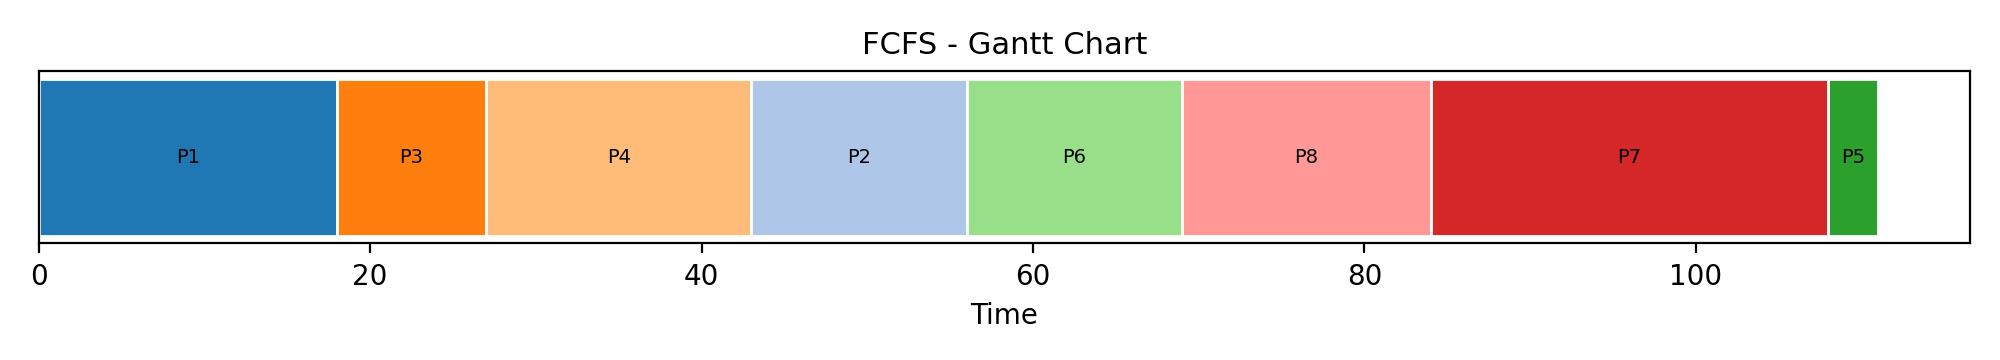
\includegraphics[width=\linewidth]{figures/gantt_fcfs.png}
  \caption{FCFS Gantt chart, small mixed workload.}
  \label{fig:gantt-fcfs}
\end{figure}
\begin{figure}[H]
  \centering
  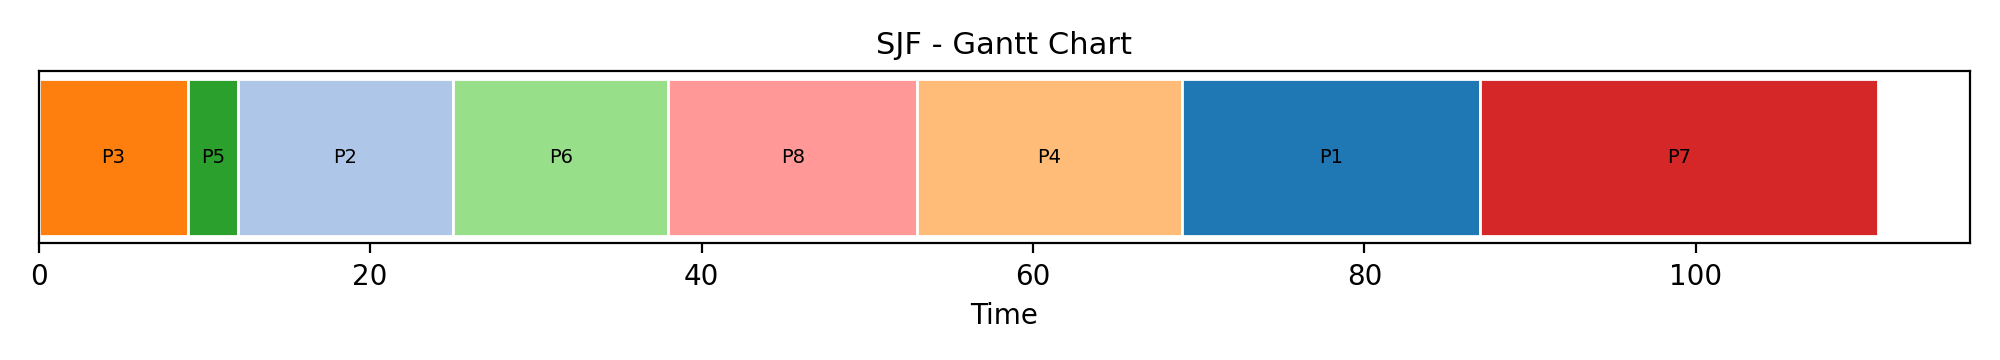
\includegraphics[width=\linewidth]{figures/gantt_sjf.png}
  \caption{SJF Gantt chart, small mixed workload.}
  \label{fig:gantt-sjf}
\end{figure}
\begin{figure}[H]
  \centering
  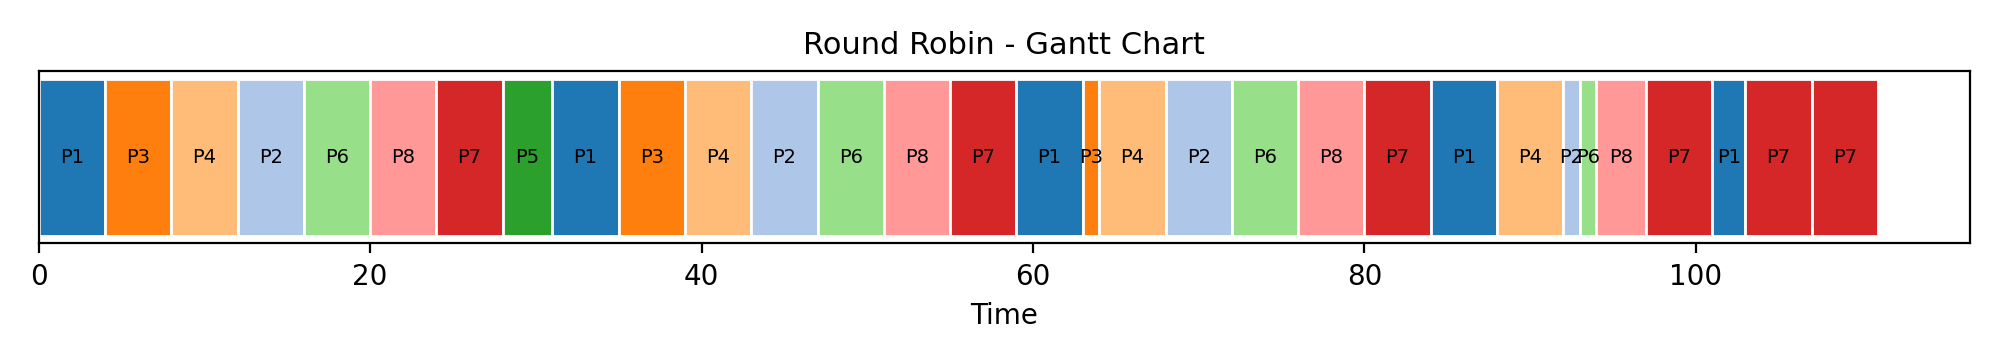
\includegraphics[width=\linewidth]{figures/gantt_round_robin.png}
  \caption{Round Robin Gantt chart (quantum=4), small mixed workload.}
  \label{fig:gantt-rr}
\end{figure}
\begin{figure}[H]
  \centering
  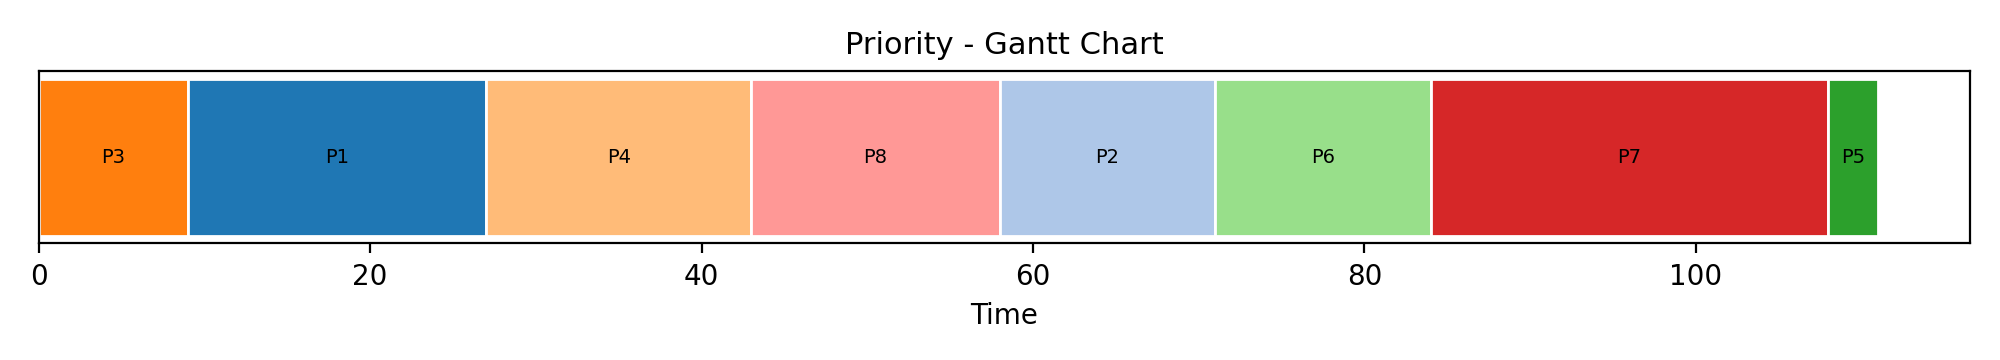
\includegraphics[width=\linewidth]{figures/gantt_priority.png}
  \caption{Priority Gantt chart, small mixed workload.}
  \label{fig:gantt-priority}
\end{figure}
\begin{figure}[H]
  \centering
  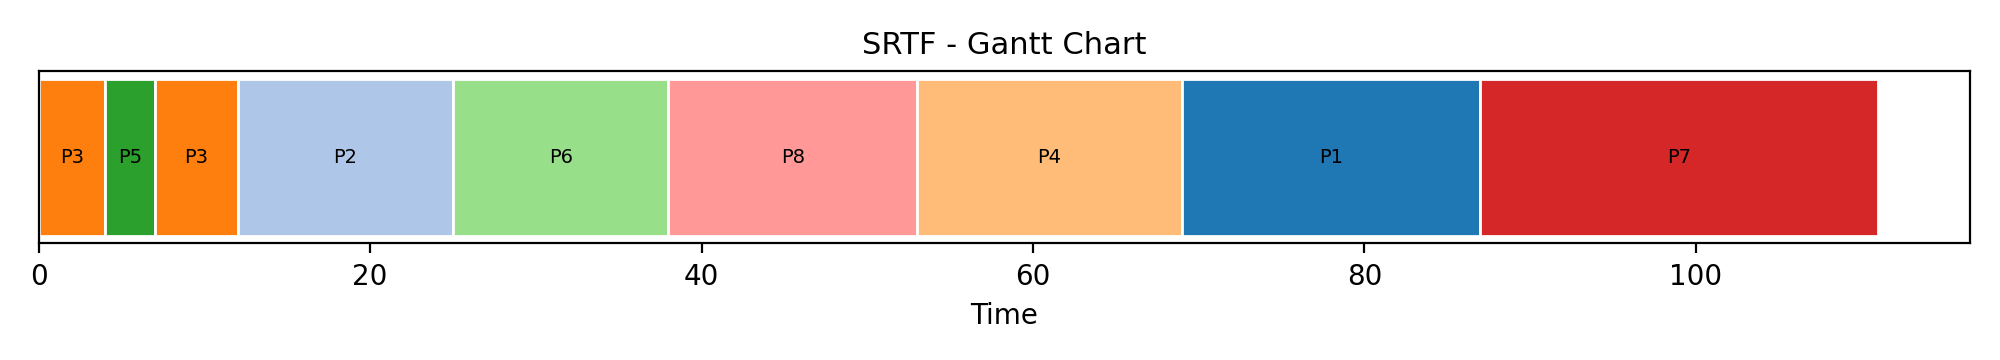
\includegraphics[width=\linewidth]{figures/gantt_srtf.png}
  \caption{SRTF Gantt chart, small mixed workload.}
  \label{fig:gantt-srtf}
\end{figure}
\begin{figure}[H]
  \centering
  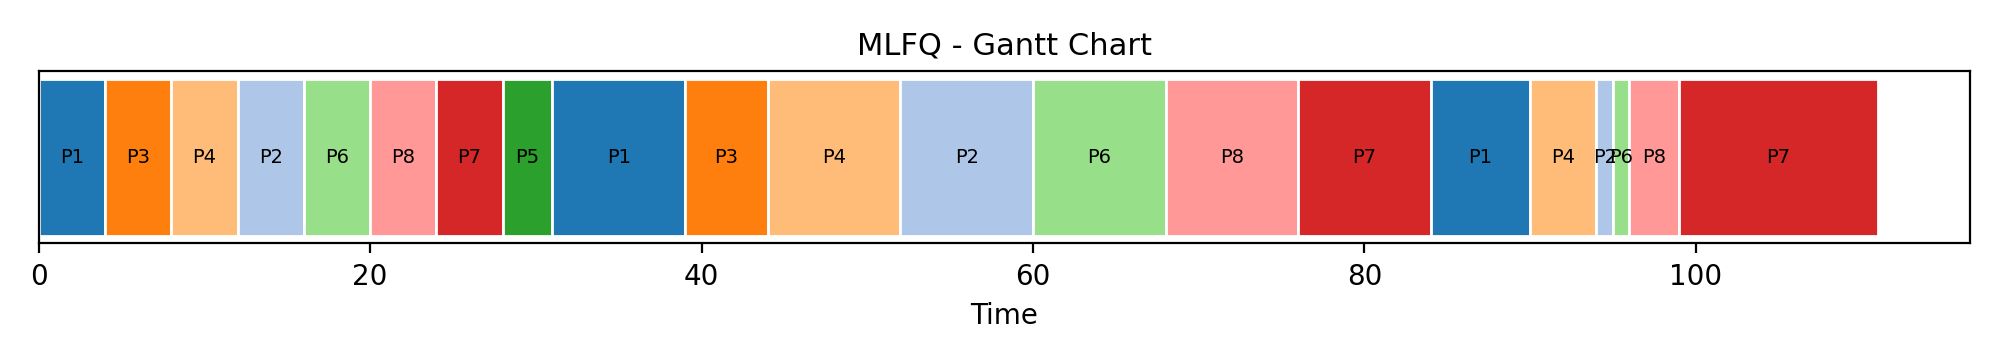
\includegraphics[width=\linewidth]{figures/gantt_mlfq.png}
  \caption{MLFQ Gantt chart (quanta=[4,8,16]), small mixed workload.}
  \label{fig:gantt-mlfq}
\end{figure}

\subsection{Algorithm Comparison Charts}

Figures~\ref{fig:compare-awt}--\ref{fig:compare-throughput} compare all six
algorithms on the medium (n=30) mixed workload, chosen as a representative
middle ground between the small and large workloads in
Section~\ref{sec:workloads}.

\begin{figure}[H]
  \centering
  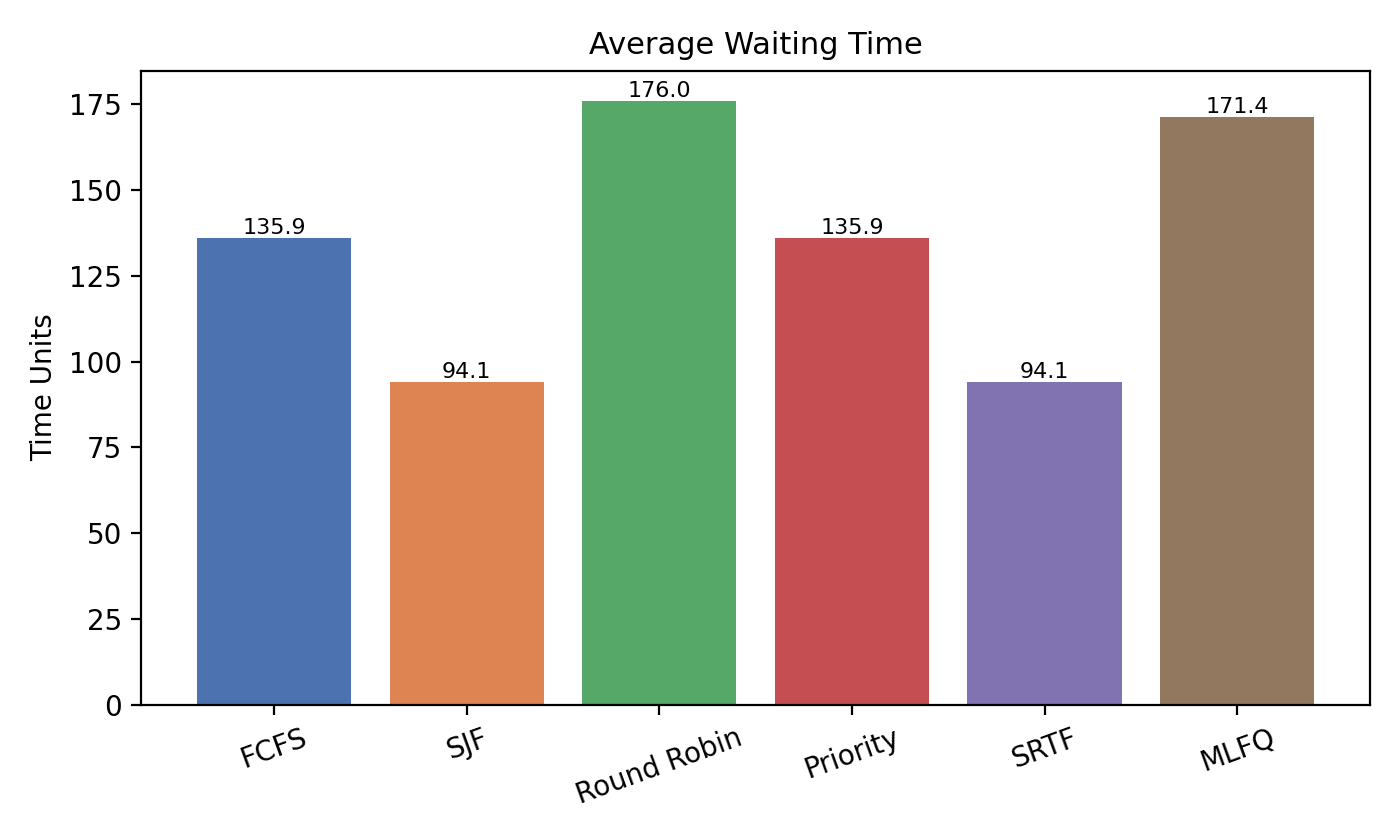
\includegraphics[width=0.85\linewidth]{figures/compare_waiting_time.png}
  \caption{Average waiting time by algorithm, medium mixed workload.}
  \label{fig:compare-awt}
\end{figure}
\begin{figure}[H]
  \centering
  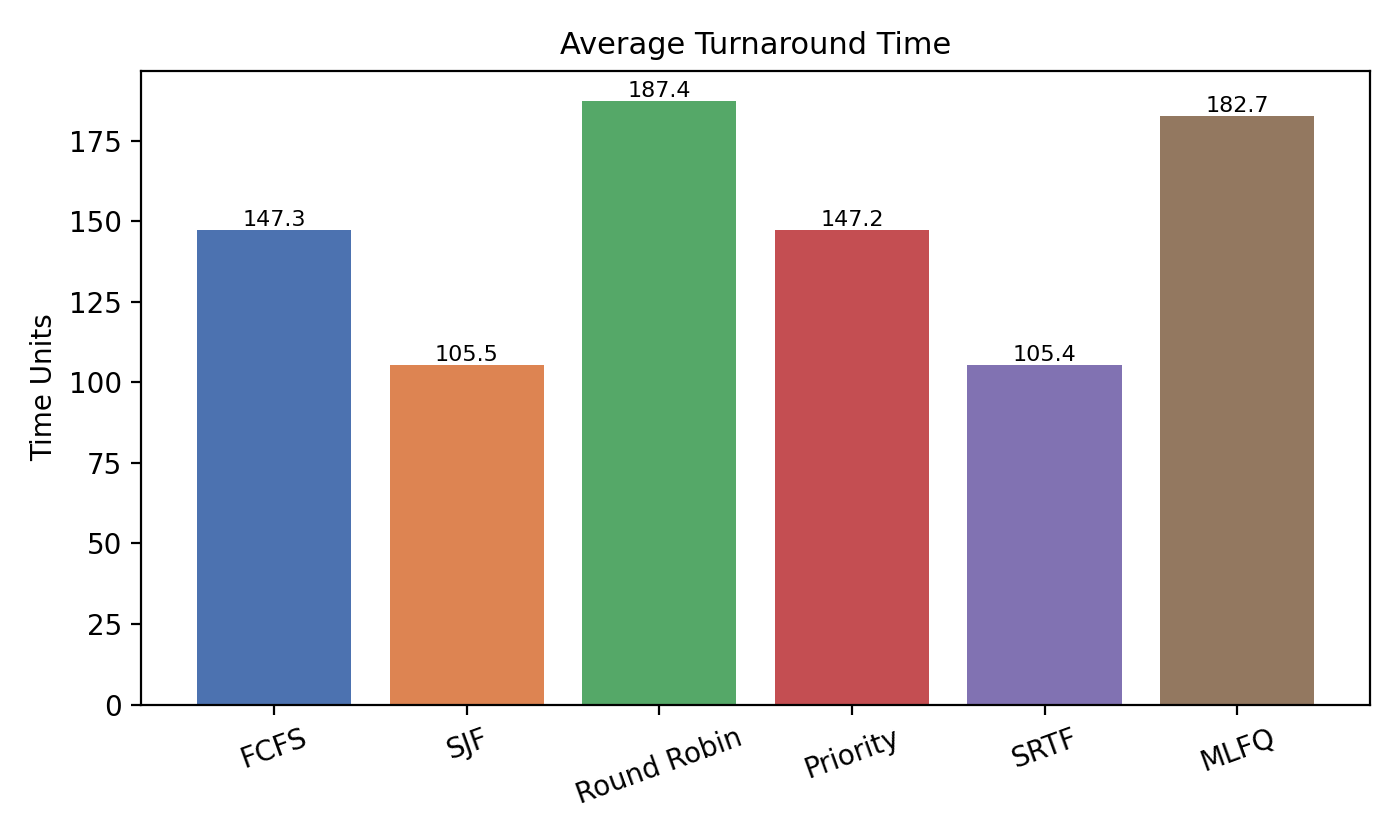
\includegraphics[width=0.85\linewidth]{figures/compare_turnaround_time.png}
  \caption{Average turnaround time by algorithm, medium mixed workload.}
  \label{fig:compare-att}
\end{figure}
\begin{figure}[H]
  \centering
  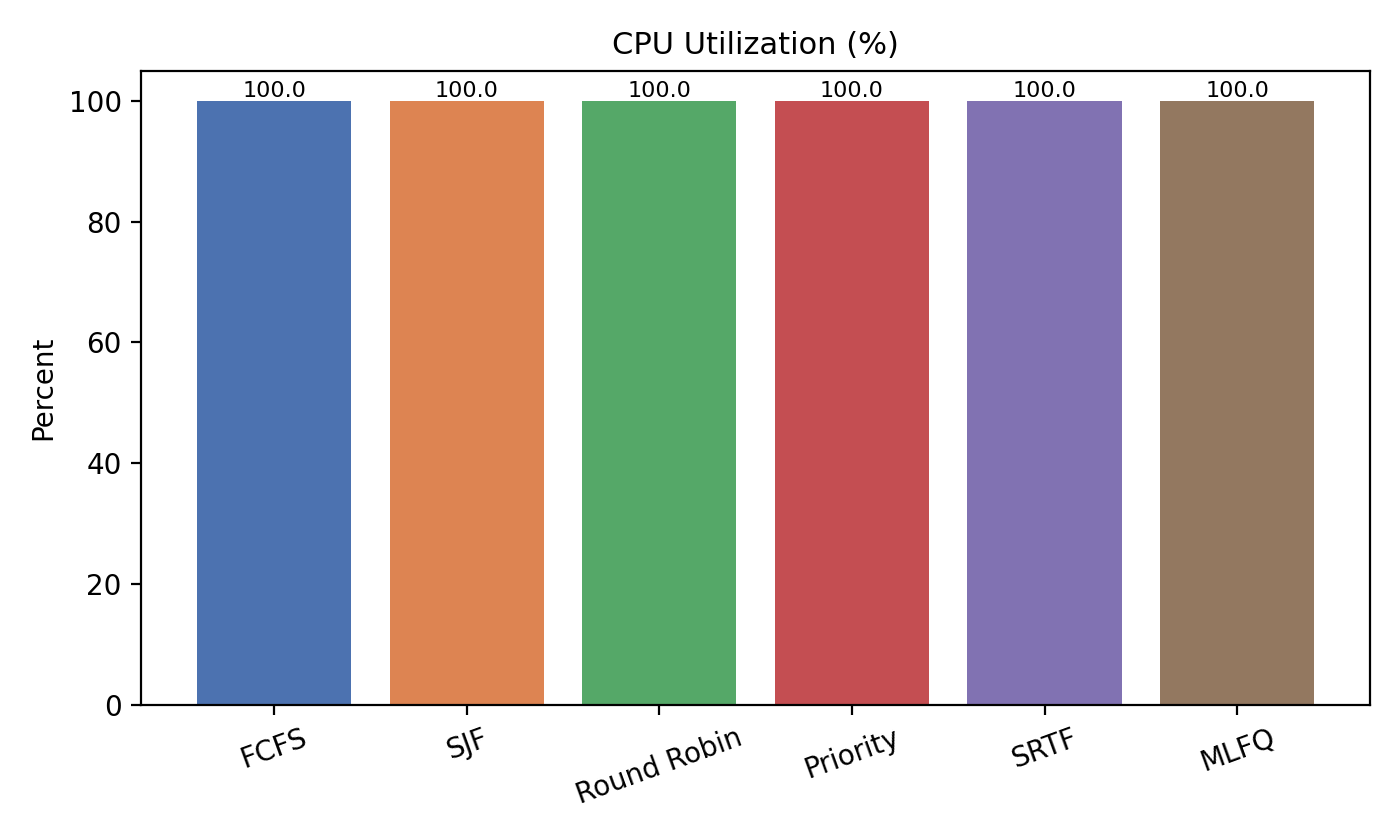
\includegraphics[width=0.85\linewidth]{figures/compare_cpu_utilization.png}
  \caption{CPU utilization by algorithm, medium mixed workload.}
  \label{fig:compare-util}
\end{figure}
\begin{figure}[H]
  \centering
  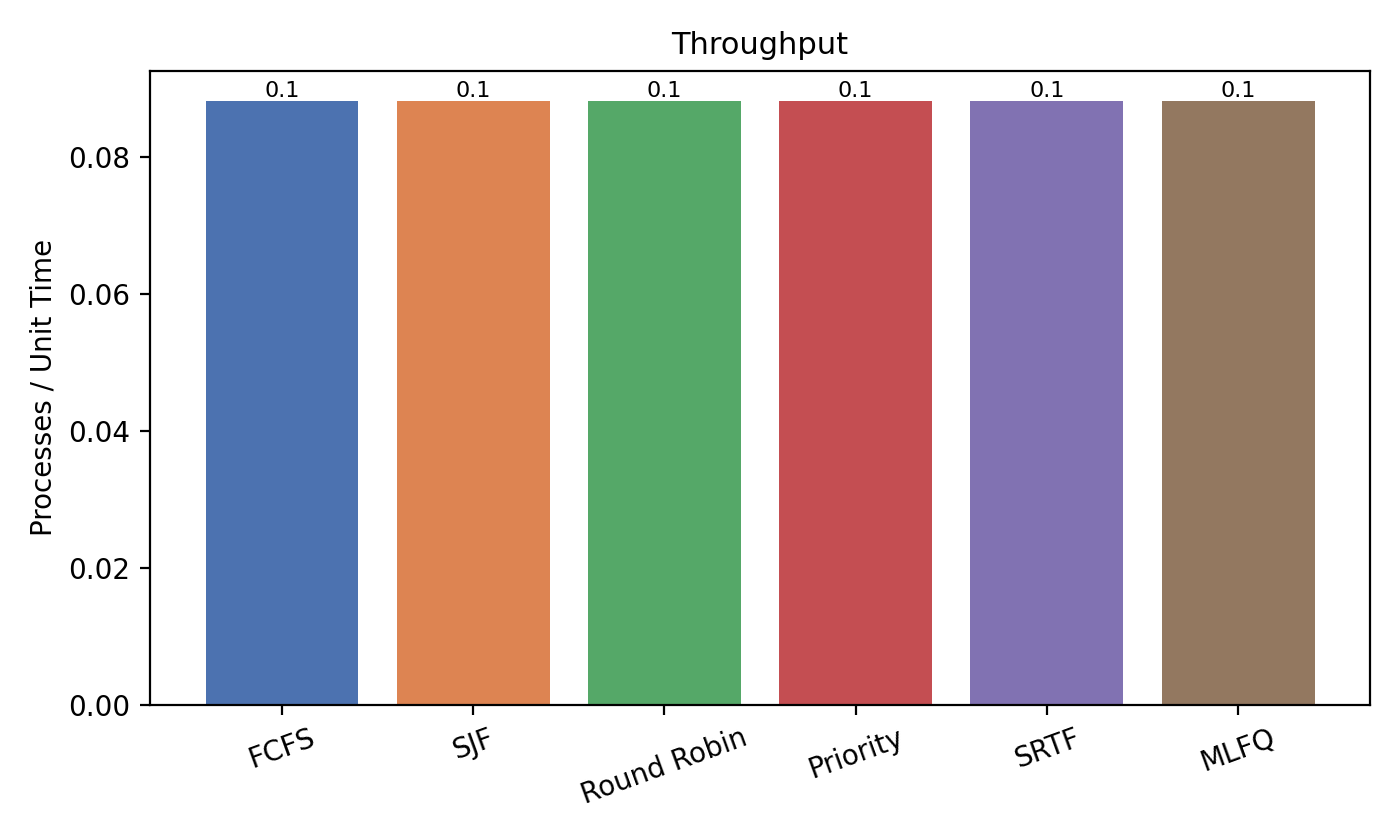
\includegraphics[width=0.85\linewidth]{figures/compare_throughput.png}
  \caption{Throughput by algorithm, medium mixed workload.}
  \label{fig:compare-throughput}
\end{figure}

\subsection{Scalability}

Figure~\ref{fig:scaling} plots average waiting time against workload size
(8, 30, 120 processes) for the mixed workload type. All algorithms scale
roughly linearly in average waiting time as load increases, which is
expected since total work grows linearly with process count on a single
CPU; the \emph{relative ordering} between algorithms (SRTF/SJF lowest,
Round Robin/MLFQ highest AWT) is preserved at every scale, which is the
more important observation for a scheduling recommendation.

\begin{figure}[H]
  \centering
  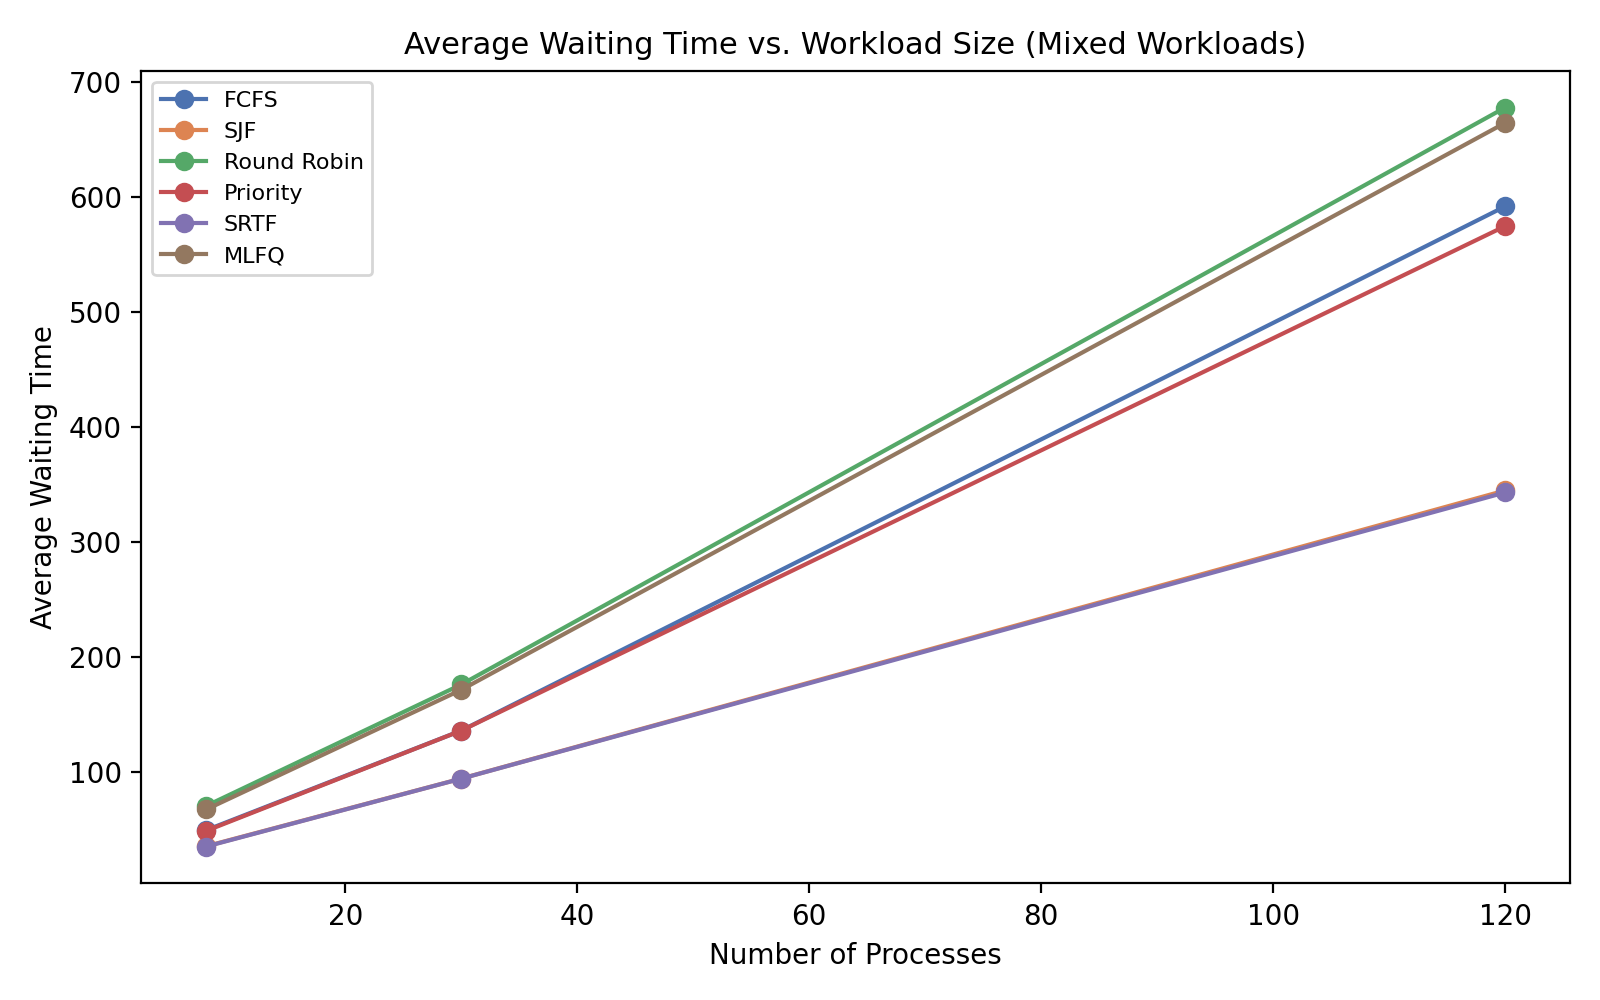
\includegraphics[width=0.9\linewidth]{figures/scaling_waiting_time.png}
  \caption{Average waiting time vs.\ workload size, mixed workloads.}
  \label{fig:scaling}
\end{figure}

% =========================================================================
\section{Discussion and Trade-offs}
\label{sec:tradeoffs}
% =========================================================================

\subsection{Waiting/Turnaround Time vs. Responsiveness}

Across every workload tested, \textbf{SRTF and SJF consistently produced
the lowest average waiting and turnaround times}, confirming the textbook
result that shortest-job-first policies (preemptive or not) are optimal
for these metrics. However, both come with the \emph{average response
time} penalty visible in the tables: because they let long jobs run once
started (SJF) or only interrupt for strictly shorter jobs (SRTF), a
process's \emph{first} CPU access can still be delayed by whatever is
currently running.

\textbf{Round Robin and MLFQ trade higher average waiting/turnaround time
for dramatically better average response time} --- both are 4--10$\times$
lower than FCFS/SJF/Priority/SRTF response time across the workloads
tested. This matches their design intent: RR and MLFQ are built for
interactive, time-sharing environments where a process getting \emph{some}
CPU quickly matters more than any one process finishing quickly.

\subsection{Practical Knowledge Requirements}

SJF and SRTF require knowing (or estimating) burst time in advance, which
is unrealistic in a general-purpose production OS. \textbf{MLFQ is the
only algorithm tested that approximates SJF/SRTF-like behavior
(favoring short jobs) without requiring advance knowledge of burst
time} --- it infers a process's nature purely from observed behavior
(whether it uses its full quantum). This is why MLFQ, despite its higher
AWT/ATT than SRTF in every table above, is the practical default in most
real operating system schedulers (a fact reflected in the historical
Unix/Windows/Linux scheduler lineage discussed in
Silberschatz et al.~\cite{silberschatz2018}).

\subsection{Starvation Risk}

Priority scheduling as implemented here has no aging mechanism, so a
continuous stream of high-priority arrivals could in principle starve a
low-priority process indefinitely. SJF and SRTF share this risk with
respect to burst time: a continuous stream of short jobs can starve a long
one. FCFS and Round Robin are starvation-free by construction --- every
process is guaranteed a bounded wait proportional to the number of other
processes in the system.

\subsection{CPU Utilization}

CPU utilization was at or near 100\% for every algorithm on every workload
tested (Table results above), which is expected: none of these workloads
include artificial idle gaps, and every algorithm here is work-conserving
(it never leaves the CPU idle while a ready process exists). Utilization
is therefore not a strongly differentiating metric for this particular
experiment; it would diverge more sharply in a workload with I/O-blocking
gaps that some schedulers handle better than others.

% =========================================================================
\section{Recommendation}
% =========================================================================

For OwlTech Industries' production systems, we recommend \textbf{MLFQ as
the default scheduler}, with the following reasoning:

\begin{enumerate}
  \item It does not require advance knowledge of process burst times,
    unlike SJF/SRTF, which is essential for a production system running
    unpredictable, user-submitted workloads.
  \item It automatically favors short/interactive processes (approximating
    SRTF's benefits) while still giving CPU-bound processes forward
    progress at a lower queue level, avoiding SJF/SRTF's starvation risk
    for long jobs.
  \item Its response-time characteristics (Table results, Section
    \ref{sec:evaluation}) are on par with Round Robin, which matters for
    any interactive or latency-sensitive workload mixed into the system.
\end{enumerate}

\textbf{Exception:} if OwlTech's workload is known in advance to be
batch-oriented with predictable burst times (e.g. a nightly ETL pipeline
with well-characterized jobs), \textbf{SRTF} should be preferred instead,
since it minimizes total waiting/turnaround time when burst times are
known and starvation of long batch jobs is an acceptable trade-off in that
context.

\textbf{Future improvements:} adding aging to the Priority and MLFQ
implementations would remove their residual starvation risk; extending the
Process model's existing \texttt{io\_bursts} field to actually alternate
CPU and I/O phases would allow CPU utilization to become a differentiating
metric, since some algorithms handle I/O-blocking gaps more efficiently
than others.

% =========================================================================
\section{Testing}
\label{sec:testing}
% =========================================================================

The test suite (\texttt{tests/test\_algorithms.py}, 36 tests) covers:

\begin{itemize}
  \item Hand-verified correctness against the assignment's own P1--P4
    example table (Section 4.1 of the assignment PDF) for FCFS, SJF,
    Round Robin, and Priority.
  \item Conservation checks: every algorithm's total executed time per
    process must equal that process's burst time.
  \item Edge cases required by the assignment: all processes arriving at
    time 0, identical burst times, and a mix of very short (1--2) and very
    long (100+) burst times.
  \item Scale checks: every algorithm against 5, 25, and 100-process
    generated workloads.
  \item Reproducibility: identical (seed, size, type) always yields an
    identical workload.
  \item Input validation: duplicate process IDs and non-positive burst
    times are rejected before simulation.
\end{itemize}

All 36 tests pass (\texttt{pytest tests/ -q} $\rightarrow$
\texttt{36 passed}).

% =========================================================================
\section{Streamlit Interface}
% =========================================================================

The web interface (\texttt{app.py}) provides an editable process table, a
workload generator (size preset, type, and seed controls), an algorithm
multiselect with Round Robin quantum and MLFQ quanta controls, a metrics
comparison table with CSV export, four algorithm-comparison bar charts,
and a per-algorithm tab with an interactive Gantt chart, full per-process
result table, and CSV export.

\begin{figure}[H]
     \centering
     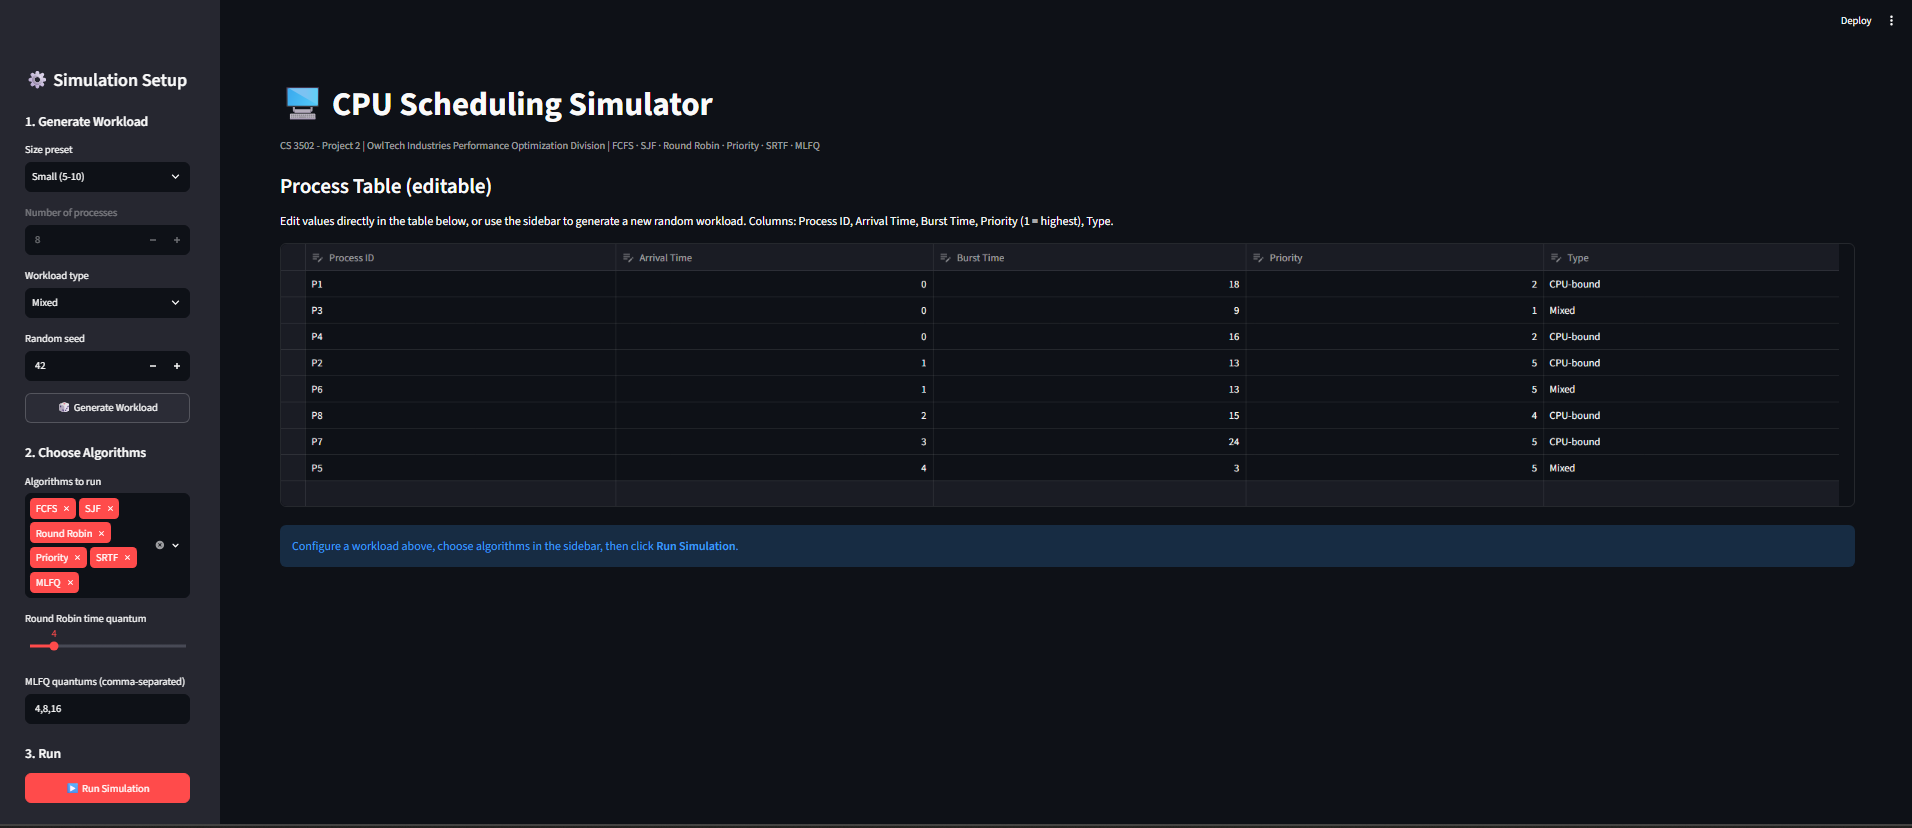
\includegraphics[width=0.9\linewidth]{figures/main_interface.png}
     \caption{Streamlit interface: process table and workload controls.}
     \label{fig:screenshot-main}
   \end{figure}

\begin{figure}[H]
     \centering
     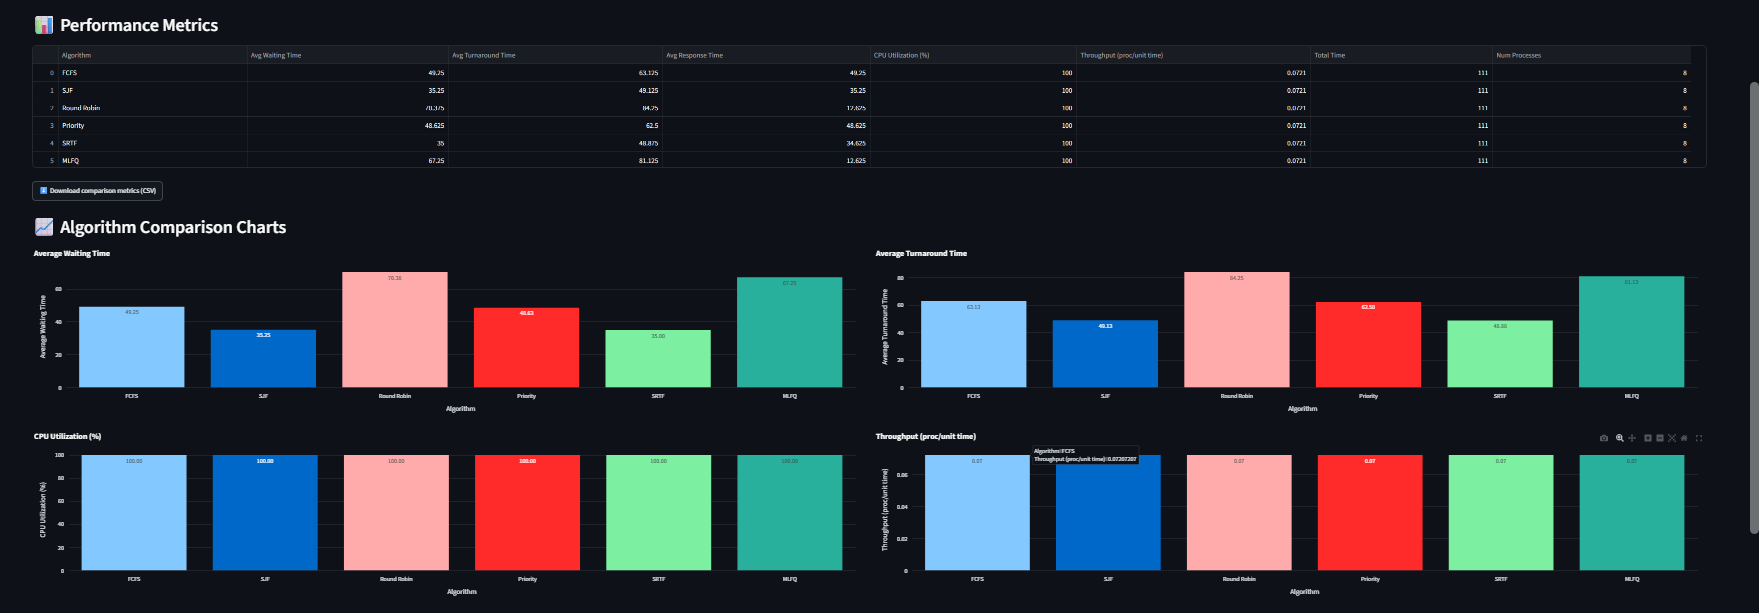
\includegraphics[width=0.9\linewidth]{figures/metrics_charts.png.png}
     \caption{Streamlit interface: performance metrics and comparison charts.}
     \label{fig:screenshot-main}
   \end{figure}

\begin{figure}[H]
     \centering
     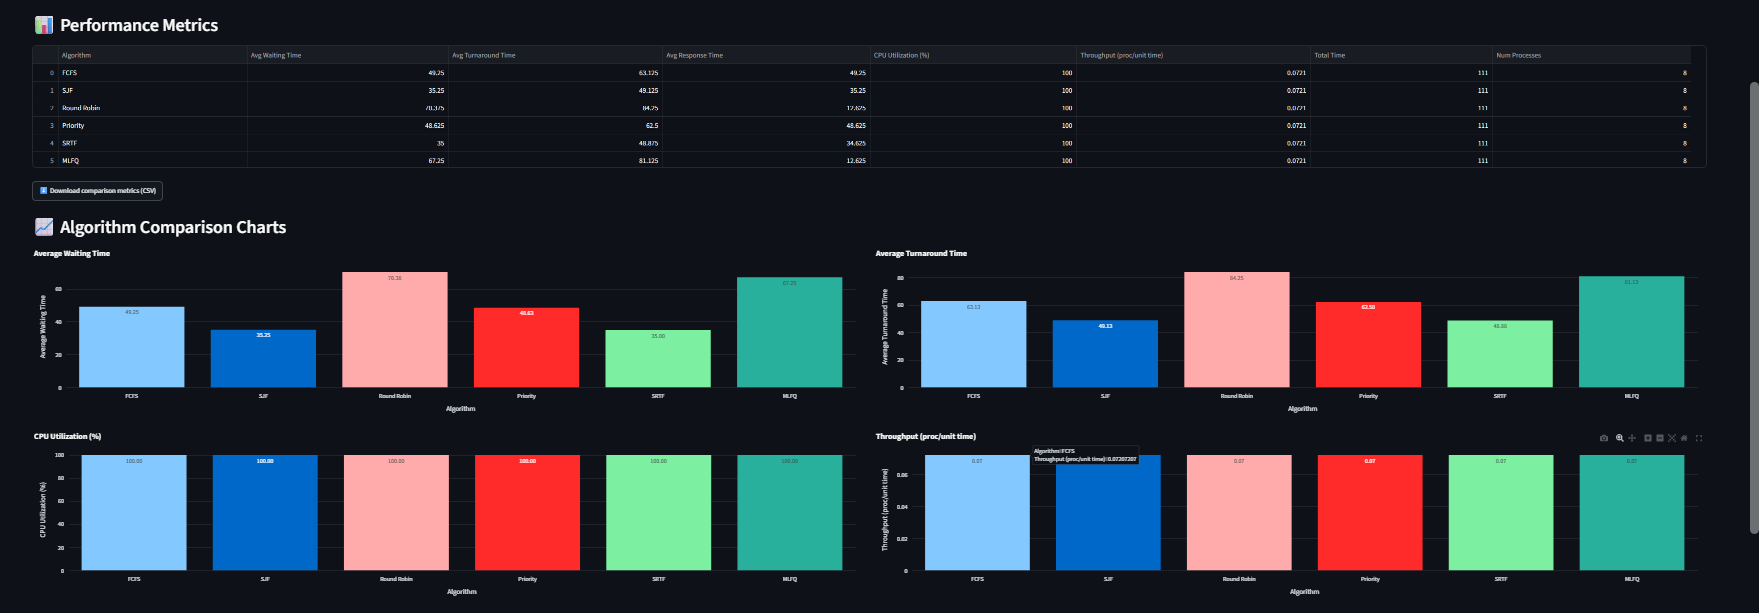
\includegraphics[width=0.9\linewidth]{figures/metrics_charts.png.png}
     \caption{Streamlit interface: interactive Gantt chart view.}
     \label{fig:screenshot-main}
   \end{figure}

% =========================================================================
\section{Conclusion}
% =========================================================================

This project implemented and empirically compared six CPU scheduling
algorithms --- FCFS, SJF, Round Robin, Priority, and the two additional
algorithms SRTF and MLFQ --- across nine workload configurations spanning
three size classes and three process-type distributions. The results
confirm the classical trade-off between minimizing average waiting/
turnaround time (best served by SRTF/SJF) and minimizing response time
(best served by Round Robin/MLFQ), and support MLFQ as the strongest
general-purpose default for a production system with unpredictable
workloads, given its lack of a starvation failure mode and its
information-free approximation of shortest-job-first behavior.

\newpage
\bibliographystyle{plain}
\bibliography{references}

\end{document}
